\documentclass[12pt,a4paper]{article}

% Packages
\usepackage[a4paper,margin=1in]{geometry}
\usepackage{titlesec}
\usepackage{longtable}
\usepackage{array}
\usepackage{enumitem}
\usepackage{graphicx}
\usepackage{hyperref}
\usepackage{xcolor}
\usepackage{fancyhdr}

% Header/Footer Configuration
\pagestyle{fancy}
\fancyhf{}
\rhead{Software Requirements Specification}
\lhead{PowerZone}
\rfoot{\thepage}

% Hyperlink Setup
\hypersetup{
    colorlinks=true,
    linkcolor=black,
    urlcolor=blue,
    pdftitle={Software Requirements Specification (SRS) - PowerZone}
}

\title{
    \textbf{Software Requirements Specification (SRS)}\\
    \vspace{0.5cm}
    \large PowerZone - Premium Gym Membership Website
}

\author{
    Prepared By: Priyanshu Jangra \\
    Department Name \\
    Institution Name
}

\date{\today}

\begin{document}

\maketitle
\tableofcontents
\newpage

% ==========================================================
\section{Introduction}

\subsection{Purpose}
The purpose of this document is to define the Software Requirements Specification (SRS) for the PowerZone platform. It details the functional and non-functional requirements, system constraints, and user interactions necessary for the successful development and deployment of the application. This document is intended for developers, project managers, QA testers, and stakeholders.

\subsection{Project Overview}
\textbf{PowerZone is a premium} fitness membership platform and web application. It bridges the gap between fragmented fitness tracking and gym discovery. The system allows users to search for nearby gyms, authenticate securely via Supabase, manage their diet and workouts through a centralized dashboard, and utilize an AI Food Scanner to estimate calories from food images.

\subsection{Scope of the Project}
The scope of PowerZone includes the development of a user-facing static application and a backend integration system.
\begin{itemize}
    \item \textbf{For Users/Members:} The system will provide a cinematic landing page, location-based gym directory, an AI food scanner, and a personalized client dashboard for tracking diet, workouts, and goals.
    \item \textbf{For System Integration:} The system will utilize Supabase for authentication and database management (PostgreSQL), along with a FastAPI backend specifically designed for Machine Learning inference (food classification).
\end{itemize}

\subsection{Objectives}
\begin{itemize}
    \item To provide an intuitive, high-end digital platform for fitness enthusiasts.
    \item To streamline the onboarding process through secure Supabase authentication.
    \item To deliver an AI-powered food scanning tool capable of accurately predicting food items and estimating macros.
    \item To digitize and organize personal fitness goals, diet plans, and gym attendance using seamless local storage integration.
\end{itemize}

\subsection{Definitions, Acronyms and Abbreviations}
\begin{longtable}{|p{3cm}|p{11cm}|}
\hline
\textbf{Term} & \textbf{Description} \\
\hline
SRS & Software Requirements Specification \\
\hline
UI/UX & User Interface / User Experience \\
\hline
BaaS & Backend as a Service (Supabase) \\
\hline
RLS & Row Level Security (Database security model) \\
\hline
ML & Machine Learning \\
\hline
JWT & JSON Web Token \\
\hline
\end{longtable}

\subsection{References}
\begin{itemize}
    \item IEEE Recommended Practice for Software Requirements Specifications (IEEE Std 830-1998).
    \item Supabase Documentation.
    \item FastAPI Documentation.
\end{itemize}

% ==========================================================
\section{Overall Description}

\subsection{System Perspective}
PowerZone is an independent, standalone web-responsive application. It operates on a decoupled architecture, where the static front-end (HTML/CSS/JS) communicates directly with a centralized BaaS (Supabase) via client-side APIs, and connects to a FastAPI server for ML predictions.

\subsection{System Features}
\begin{itemize}
    \item \textbf{Authentication System:} Secure email/password registration, login, and password reset flows with auto-profile generation.
    \item \textbf{Client Dashboard:} Multi-panel dashboard for managing Diet, Workouts, Goals, and Calendar attendance.
    \item \textbf{AI Food Scanner:} Image upload interface interacting with Indian and Global ML models to predict food and calculate calories.
    \item \textbf{Gym Directory:} Searchable, filterable directory of local fitness centers with Google Maps navigation.
    \item \textbf{Franchise Portal:} Informational section for prospective partners to apply for a PowerZone franchise.
\end{itemize}

\subsection{User Classes and Characteristics}
\begin{longtable}{|p{4cm}|p{10cm}|}
\hline
\textbf{User Type} & \textbf{Responsibilities} \\
\hline
Visitor & Can browse the landing page, search the gym directory, test the AI scanner, and view the franchise portal. \\
\hline
Authenticated Member & Has access to the protected client dashboard to manage daily diets, track workouts, and log gym attendance. \\
\hline
System Administrator & Manages Supabase configuration, RLS policies, ML server uptime, and user database health. \\
\hline
\end{longtable}

\subsection{Operating Environment}
\begin{itemize}
    \item \textbf{Web Interface:} Compatible with modern web browsers (Google Chrome, Mozilla Firefox, Apple Safari, Microsoft Edge).
    \item \textbf{Backend / Database:} Supabase Cloud Infrastructure (PostgreSQL).
    \item \textbf{ML Engine:} Python FastAPI server running classification models.
\end{itemize}

\subsection{Design and Implementation Constraints}
\begin{itemize}
    \item \textbf{Framework Constraint:} The frontend must be developed without external frameworks (No React, Vue, etc.)—relying purely on HTML5, CSS3, and Vanilla JavaScript.
    \item \textbf{State Management:} The Client Dashboard heavily relies on \texttt{localStorage} to persist the state of goals and workouts.
    \item \textbf{API Dependency:} The AI Scanner requires a live connection to the FastAPI backend to function.
\end{itemize}

\subsection{Assumptions and Dependencies}
\begin{itemize}
    \item \textbf{Assumptions:} Users must have an active internet connection to authenticate and use the ML features. 
    \item \textbf{Dependencies:} The application relies on Supabase for BaaS functionality, and Google Maps API for gym mapping features.
\end{itemize}

% ==========================================================
\section{Problem Statement}

\subsection{Existing System}
Currently, fitness enthusiasts rely on multiple fragmented applications. They use one application to scan or log their daily food intake (such as MyFitnessPal), a separate spreadsheet or app to log their daily gym routines, and external search engines to find gyms or subscription plans. 

\subsection{Problems Identified}
\begin{itemize}
    \item \textbf{Fragmented Experience:} Users are forced to switch between multiple apps to manage their fitness lifestyle.
    \item \textbf{Manual Food Logging:} Entering food ingredients manually is tedious, inaccurate, and discouraging for users.
    \item \textbf{Lack of Premium Aesthetics:} Many fitness platforms have cluttered UIs that do not inspire motivation or provide a high-end luxury feel.
\end{itemize}

\subsection{Proposed Solution}
PowerZone proposes an all-in-one, premium fitness platform. By integrating a seamless dashboard for diet and workout tracking with a cutting-edge AI Food Scanner, PowerZone eliminates the need for multiple apps. Furthermore, its luxury dark-mode aesthetic provides an inspiring, Equinox-style digital experience.

% ==========================================================
\section{Functional Requirements}

\subsection{Module 1: Authentication System}
\begin{itemize}
    \item \textbf{User Registration:} The system shall allow users to register by providing their Full Name, Email, Password, and accepting the terms.
    \item \textbf{Login \& Verification:} Secure login using email and password via Supabase Auth. It must support a secure password reset flow through recovery emails.
    \item \textbf{Profile Creation:} A database trigger shall automatically create a row in the \texttt{public.profiles} table whenever a new user signs up in \texttt{auth.users}.
\end{itemize}

\subsection{Module 2: Client Dashboard}
\begin{itemize}
    \item \textbf{Diet \& Gym Tracking:} The dashboard must allow users to generate diet plans, add meals, and track daily workout sessions.
    \item \textbf{Goal Management:} Users must be able to add, achieve, or remove custom fitness goals.
    \item \textbf{Calendar System:} A visual calendar where users can mark their gym attendance.
\end{itemize}

\subsection{Module 3: AI Food Scanner}
\begin{itemize}
    \item \textbf{Image Processing:} The system shall allow users to upload images of their food.
    \item \textbf{ML Inference:} Images must be transmitted to the FastAPI backend, which will utilize both Indian and Global ML models.
    \item \textbf{Results Output:} The system shall display the predicted food label, estimated calories, macros, and AI confidence score.
\end{itemize}

\subsection{Module 4: Gym Discovery}
\begin{itemize}
    \item \textbf{Gym Directory:} An interactive listing of local gyms with capabilities to filter by category and location.
    \item \textbf{Gym Profiles:} Detailed views of specific gyms (e.g., Forge Fitness) showing subscription plans and map navigation.
\end{itemize}

% ==========================================================
\section{Non-Functional Requirements}

\subsection{Performance Requirements}
\begin{itemize}
    \item \textbf{Response Time:} The static frontend must achieve a near-instant Time-To-Interactive (TTI). The AI scanner must return inference results within 3 seconds.
    \item \textbf{Concurrency:} Supabase must handle multiple concurrent user logins efficiently.
\end{itemize}

\subsection{Security Requirements}
\begin{itemize}
    \item \textbf{Data Protection:} Row Level Security (RLS) policies must be strictly enforced on the Postgres database to ensure users can only read/update their own profile data.
    \item \textbf{Secure Communication:} All authentication requests to Supabase and image uploads to FastAPI must be encrypted over HTTPS.
\end{itemize}

\subsection{Reliability Requirements}
\begin{itemize}
    \item \textbf{Uptime:} The platform relies on Supabase and Vercel/Netlify, targeting 99.9\% uptime.
    \item \textbf{State Recovery:} Dashboard state is saved to \texttt{localStorage}, ensuring data is retained across sessions on the same device.
\end{itemize}

\subsection{Usability Requirements}
\begin{itemize}
    \item \textbf{Intuitive UI:} A cinematic, dark-themed interface with glassmorphism, parallax effects, and smooth micro-animations.
    \item \textbf{Accessibility:} Despite the dark theme, contrast ratios must be maintained to ensure readable text.
\end{itemize}

\subsection{Maintainability Requirements}
\begin{itemize}
    \item \textbf{Code Architecture:} The frontend uses standard HTML/CSS/JS without complex build steps, ensuring ease of maintenance.
    \item \textbf{API Structure:} The FastAPI backend must validate inputs cleanly before routing to the ML models.
\end{itemize}

\subsection{Portability Requirements}
\begin{itemize}
    \item \textbf{Cross-Platform Support:} Fully responsive across desktop, tablet, and mobile browsers.
\end{itemize}

% ==========================================================
\section{System Architecture}

\subsection{Architecture Diagram}
\vspace{0.5cm}
\begin{figure}[h]
\centering
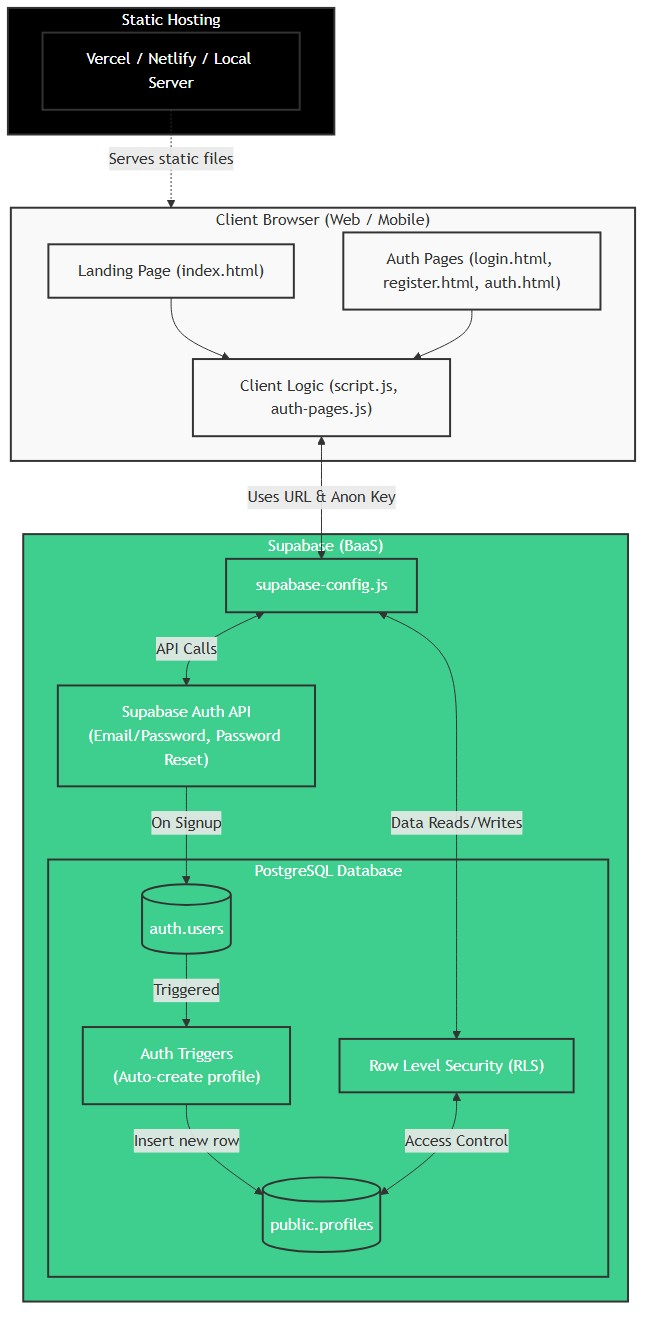
\includegraphics[width=0.9\textwidth]{HLD.jpg}
\vspace{0.3cm}
\caption{System Architecture Diagram (High Level Design)}
\end{figure}
\vspace{0.5cm}

\subsection{Architecture Description}
The PowerZone platform utilizes a \textbf{Decoupled Serverless Architecture}. 
\begin{itemize}
    \item \textbf{Client-Side:} Static assets (HTML, CSS, JS) served globally via CDN. It handles all UI rendering, layout animations, and dashboard state management (via localStorage).
    \item \textbf{Authentication \& Database (Supabase):} Acts as the primary backend. The frontend communicates directly with Supabase via its JS SDK to handle user sessions and query the PostgreSQL database.
    \item \textbf{Machine Learning API (FastAPI):} An isolated microservice that receives image payloads, runs them through pre-trained PyTorch/TensorFlow models, and returns JSON nutritional data.
\end{itemize}

\vspace{0.5cm}
\begin{figure}[h]
\centering
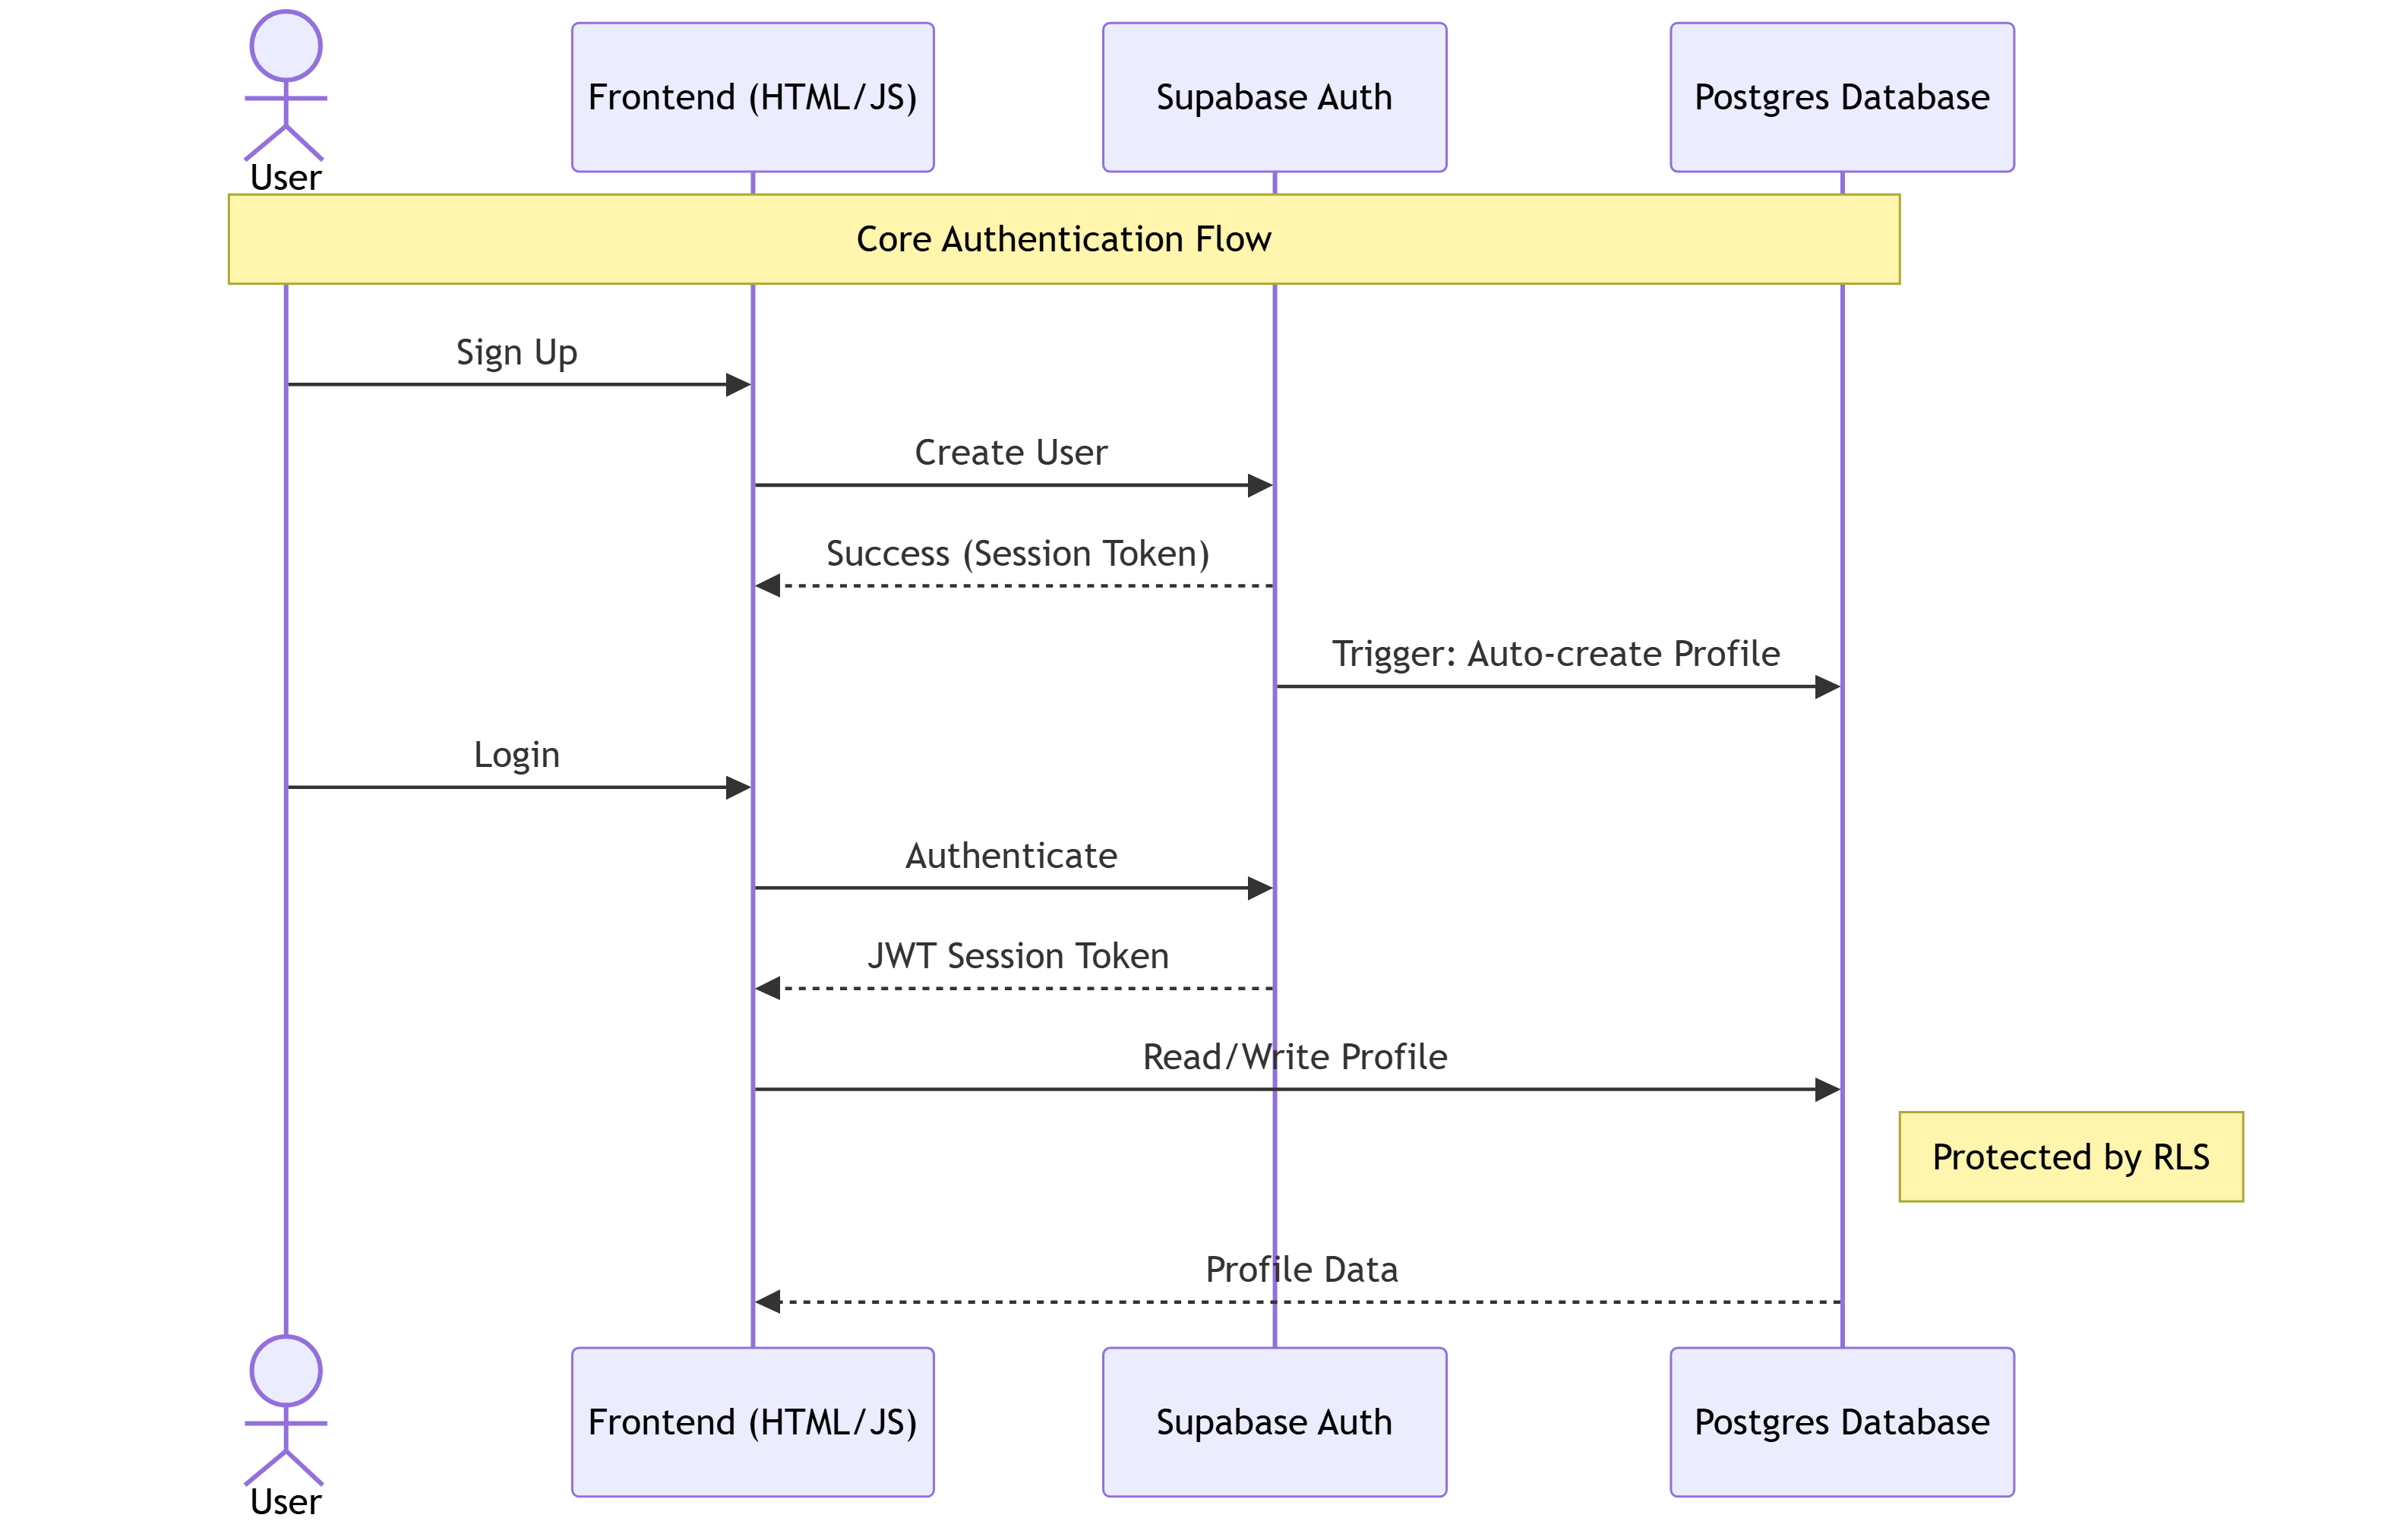
\includegraphics[width=0.9\textwidth]{lld-short.png}
\vspace{0.3cm}
\caption{Low Level Design Diagram}
\end{figure}
\vspace{0.5cm}

% ==========================================================
\section{Database Design}

\subsection{Database Tables}
\begin{longtable}{|p{3cm}|p{6cm}|p{5cm}|}
\hline
\textbf{Table Name} & \textbf{Attributes} & \textbf{Description} \\
\hline
auth.users & id (UUID), email, encrypted\_password, created\_at & Managed by Supabase internally for secure authentication. \\
\hline
public.profiles & id (UUID, PK), updated\_at, full\_name, avatar\_url & Stores public-facing user profile information. Automatically generated via SQL triggers. \\
\hline
\end{longtable}

% ==========================================================
\section{API Specifications}

\subsection{Authentication APIs (Supabase)}
These methods are executed via the Supabase JavaScript Client.
\begin{itemize}
    \item \textbf{signUp()}
    \begin{itemize}
        \item Description: Creates a new user account.
        \item Payload: \texttt{\{ "email", "password", "options": \{ "data": \{"full\_name"\} \} \}}
    \end{itemize}
    \item \textbf{signInWithPassword()}
    \begin{itemize}
        \item Description: Authenticates a user and establishes a secure session.
    \end{itemize}
    \item \textbf{resetPasswordForEmail()}
    \begin{itemize}
        \item Description: Triggers a password recovery email.
    \end{itemize}
\end{itemize}

\subsection{Machine Learning APIs}
\begin{itemize}
    \item \textbf{POST /api/scan-food}
    \begin{itemize}
        \item Description: Processes a food image to classify its contents and estimate macros.
        \item Payload: \texttt{multipart/form-data} containing the image file.
        \item Response: \texttt{\{ "calories": int, "label": string, "confidence": float, "model\_used": string \}}
    \end{itemize}
\end{itemize}

% ==========================================================
\section{User Interface Design}

\subsection{Wireframes \& Layout}
The PowerZone UI is designed with a dark, cinematic aesthetic.
\begin{itemize}
    \item \textbf{Navigation:} Transparent glassmorphic navbar with a pill-shaped container and glossy hover effects.
    \item \textbf{Hero Section:} Full-viewport background with parallax scrolling and bold typography ("NO HESITATION. FULL COMMITMENT.").
    \item \textbf{Feature Cards:} Clean, contrasting design presenting services like FITPASS, FITCOACH, FITFEAST, and FITPASS-TV.
\end{itemize}

\subsection{Page Descriptions}
\textbf{Landing Page (index.html)}\\
Showcases the premium brand, feature timeline cards, app preview mockups, and routes to sub-pages.

\textbf{Auth Pages (login.html, register.html, auth.html)}\\
Dedicated, cleanly styled pages handling the full Supabase authentication lifecycle, including password resets.

\textbf{Client Dashboard (client.html)}\\
The protected area where authenticated users manage their fitness journey. Panels are dedicated to Diet, Workouts, Goals, and Calendar.

\textbf{Health Stream (health-stream.html)}\\
The interface for the AI Food Scanner, allowing users to upload images and view nutritional inferences.

% ==========================================================
\section{Use Case Diagrams}

\subsection{Use Case Flow}
\vspace{0.5cm}
\begin{figure}[h]
\centering
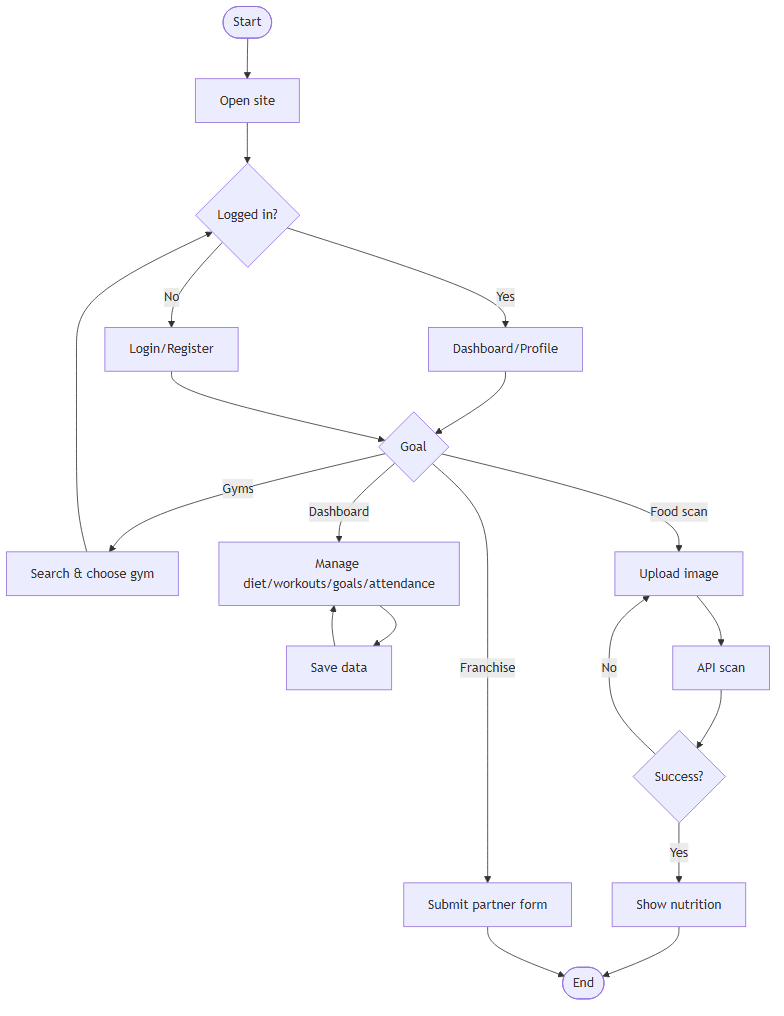
\includegraphics[width=0.8\textwidth]{powerzone-flowchart.png}
\vspace{0.3cm}
\caption{System Flowchart Diagram}
\end{figure}
\vspace{0.5cm}

\subsection{Use Case Descriptions}
\begin{longtable}{|p{4cm}|p{10cm}|}
\hline
\textbf{Use Case} & \textbf{Description} \\
\hline
User Registration & Visitor creates an account, triggering a profile creation in the database. \\
\hline
Manage Dashboard & Member updates workout status and diet logs, saving state locally. \\
\hline
Scan Food Image & Member uploads food image; backend returns macro estimations. \\
\hline
Browse Gyms & Visitor filters and views local gym subscription options. \\
\hline
\end{longtable}

% ==========================================================
\section{Activity and Sequence Diagrams}

\subsection{Sequence Diagram}
\vspace{0.5cm}
\begin{figure}[h]
\centering
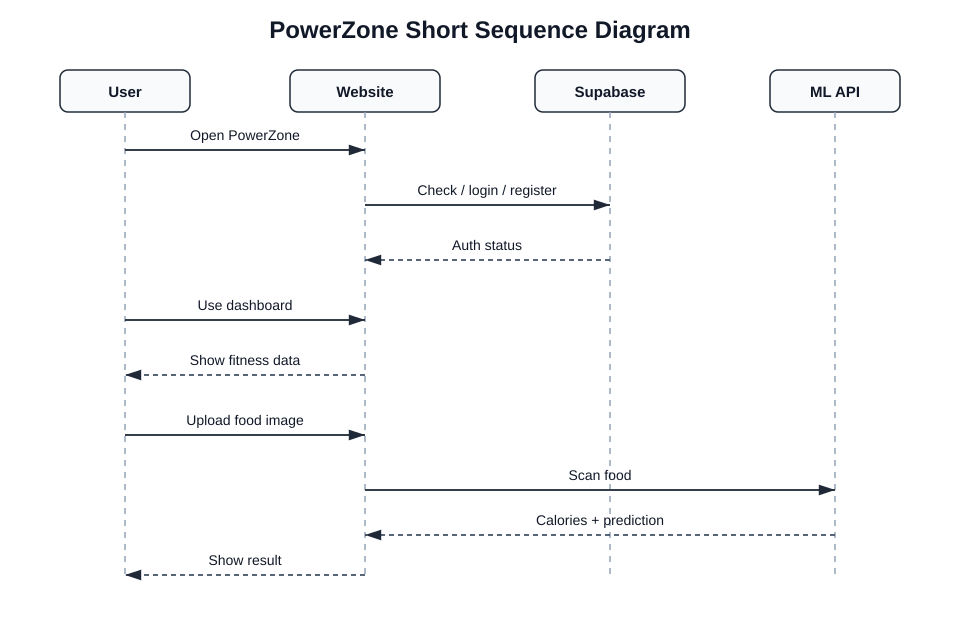
\includegraphics[width=0.9\textwidth]{short_sequence_diagram.svg}
\vspace{0.3cm}
\caption{System Sequence Diagram}
\end{figure}
\vspace{0.5cm}

% ==========================================================
\section{Testing Requirements}

\subsection{Testing Strategy}
\begin{enumerate}
    \item \textbf{UI/UX Testing:} Verify parallax scrolling, glassmorphism rendering, and responsiveness across major browsers.
    \item \textbf{Integration Testing:} Test Supabase API flows to ensure users cannot access the dashboard without a valid session token.
    \item \textbf{ML API Testing:} Send various food images (clear, blurry, dark) to the FastAPI endpoint to ensure robust error handling and acceptable confidence scores.
\end{enumerate}

\subsection{Test Cases}
\begin{longtable}{|p{2cm}|p{6cm}|p{6cm}|}
\hline
\textbf{Test ID} & \textbf{Test Scenario} & \textbf{Expected Result} \\
\hline
TC01 & Valid Login & User is redirected to Client Dashboard. \\
\hline
TC02 & Invalid Login & UI displays authentication error. \\
\hline
TC03 & Food Scan (Valid) & Returns JSON with calories and food label. \\
\hline
TC04 & RLS Enforcement & User A cannot update User B's profile row. \\
\hline
TC05 & Dashboard State & Refreshing the page retains local goals/diets. \\
\hline
\end{longtable}

% ==========================================================
\section{Deployment Requirements}

\subsection{Deployment Architecture}
\begin{itemize}
    \item \textbf{Frontend Application:} Hosted via static hosting platforms (Vercel, Netlify, or GitHub Pages).
    \item \textbf{Database \& Auth:} Supabase Cloud Platform.
    \item \textbf{ML Backend:} Python FastAPI server deployed on Render, Railway, or AWS EC2.
\end{itemize}

\subsection{Software Requirements}
\begin{itemize}
    \item \textbf{Frontend:} HTML5, CSS3, Vanilla JavaScript
    \item \textbf{Backend / DB:} PostgreSQL (Supabase)
    \item \textbf{Machine Learning:} Python 3.9+, FastAPI, PyTorch/TensorFlow
\end{itemize}

% ==========================================================
\section{Project Planning and Timeline}

\subsection{Development Methodology}
The project follows an iterative prototyping methodology, focusing heavily on front-end aesthetics and UI/UX first, followed by Supabase backend integration, and concluding with the deployment of the isolated Machine Learning API.

\subsection{Milestones}
\begin{longtable}{|p{5cm}|p{4cm}|p{3cm}|}
\hline
\textbf{Phase} & \textbf{Duration} & \textbf{Status} \\
\hline
UI/UX Design \& Static Pages & 2 Weeks & DONE \\
\hline
Supabase Integration & 1 Week & DONE \\
\hline
ML API Development & 2 Weeks & Pending \\
\hline
End-to-End Testing & 1 Week & Pending \\
\hline
Final Deployment & 1 Week & Pending \\
\hline
\end{longtable}

% ==========================================================
\section{Future Enhancements}
\begin{itemize}
    \item Migration of Dashboard \texttt{localStorage} to Supabase Postgres to enable cross-device synchronization.
    \item Integration of Stripe for real gym subscription payments.
    \item Expansion of ML models for enhanced accuracy across diverse global cuisines.
\end{itemize}

% ==========================================================
\section{Risk Analysis}
\begin{itemize}
    \item \textbf{Technical Risk:} FastAPI inference server may experience latency under high concurrent load due to heavy ML model processing. Mitigation: Implement queueing or deploy on GPU-backed instances.
    \item \textbf{Security Risk:} Exposure of Supabase Anon Keys. Mitigation: Strict RLS policy enforcement.
\end{itemize}

% ==========================================================
\section{Conclusion}
PowerZone represents a leap forward in digital fitness platforms, combining high-end aesthetic design with practical utility. By offering a unified dashboard for daily tracking, robust authentication, and an innovative AI Food Scanner, it provides users with the tools they need to achieve full commitment to their fitness goals.

% ==========================================================
\section{Appendix}

\subsection{Glossary}
\begin{longtable}{|p{3cm}|p{11cm}|}
\hline
Supabase & Open-source Firebase alternative providing Postgres DB and Auth. \\
\hline
FastAPI & Modern, fast web framework for building APIs with Python. \\
\hline
RLS & Row Level Security, ensuring users can only access their authorized data. \\
\hline
\end{longtable}

\subsection{Sample Screenshots}
\textit{Note: The exact mockups and UI captures from the PowerZone project will be included here to demonstrate the cinematic hero section, glassmorphic navigation, and dashboard interface.}

\begin{figure}[h]
\centering
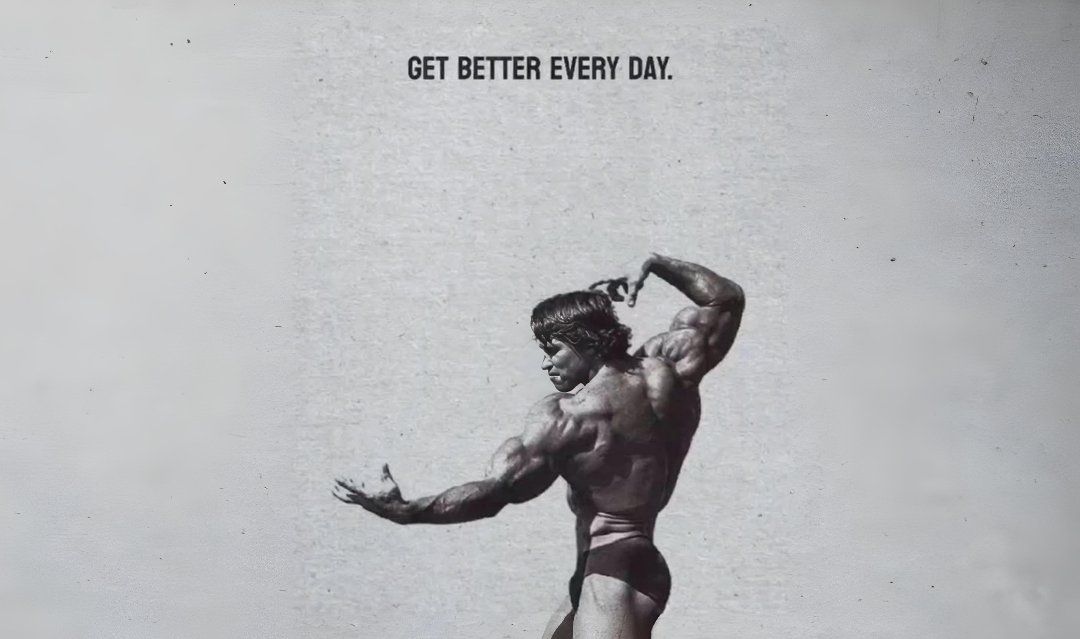
\includegraphics[width=0.9\textwidth]{../frontend/images/day gym.jpg}
\vspace{0.3cm}
\caption{PowerZone Hero Section / Main Interface}
\end{figure}
\vspace{0.5cm}

\begin{figure}[h]
\centering
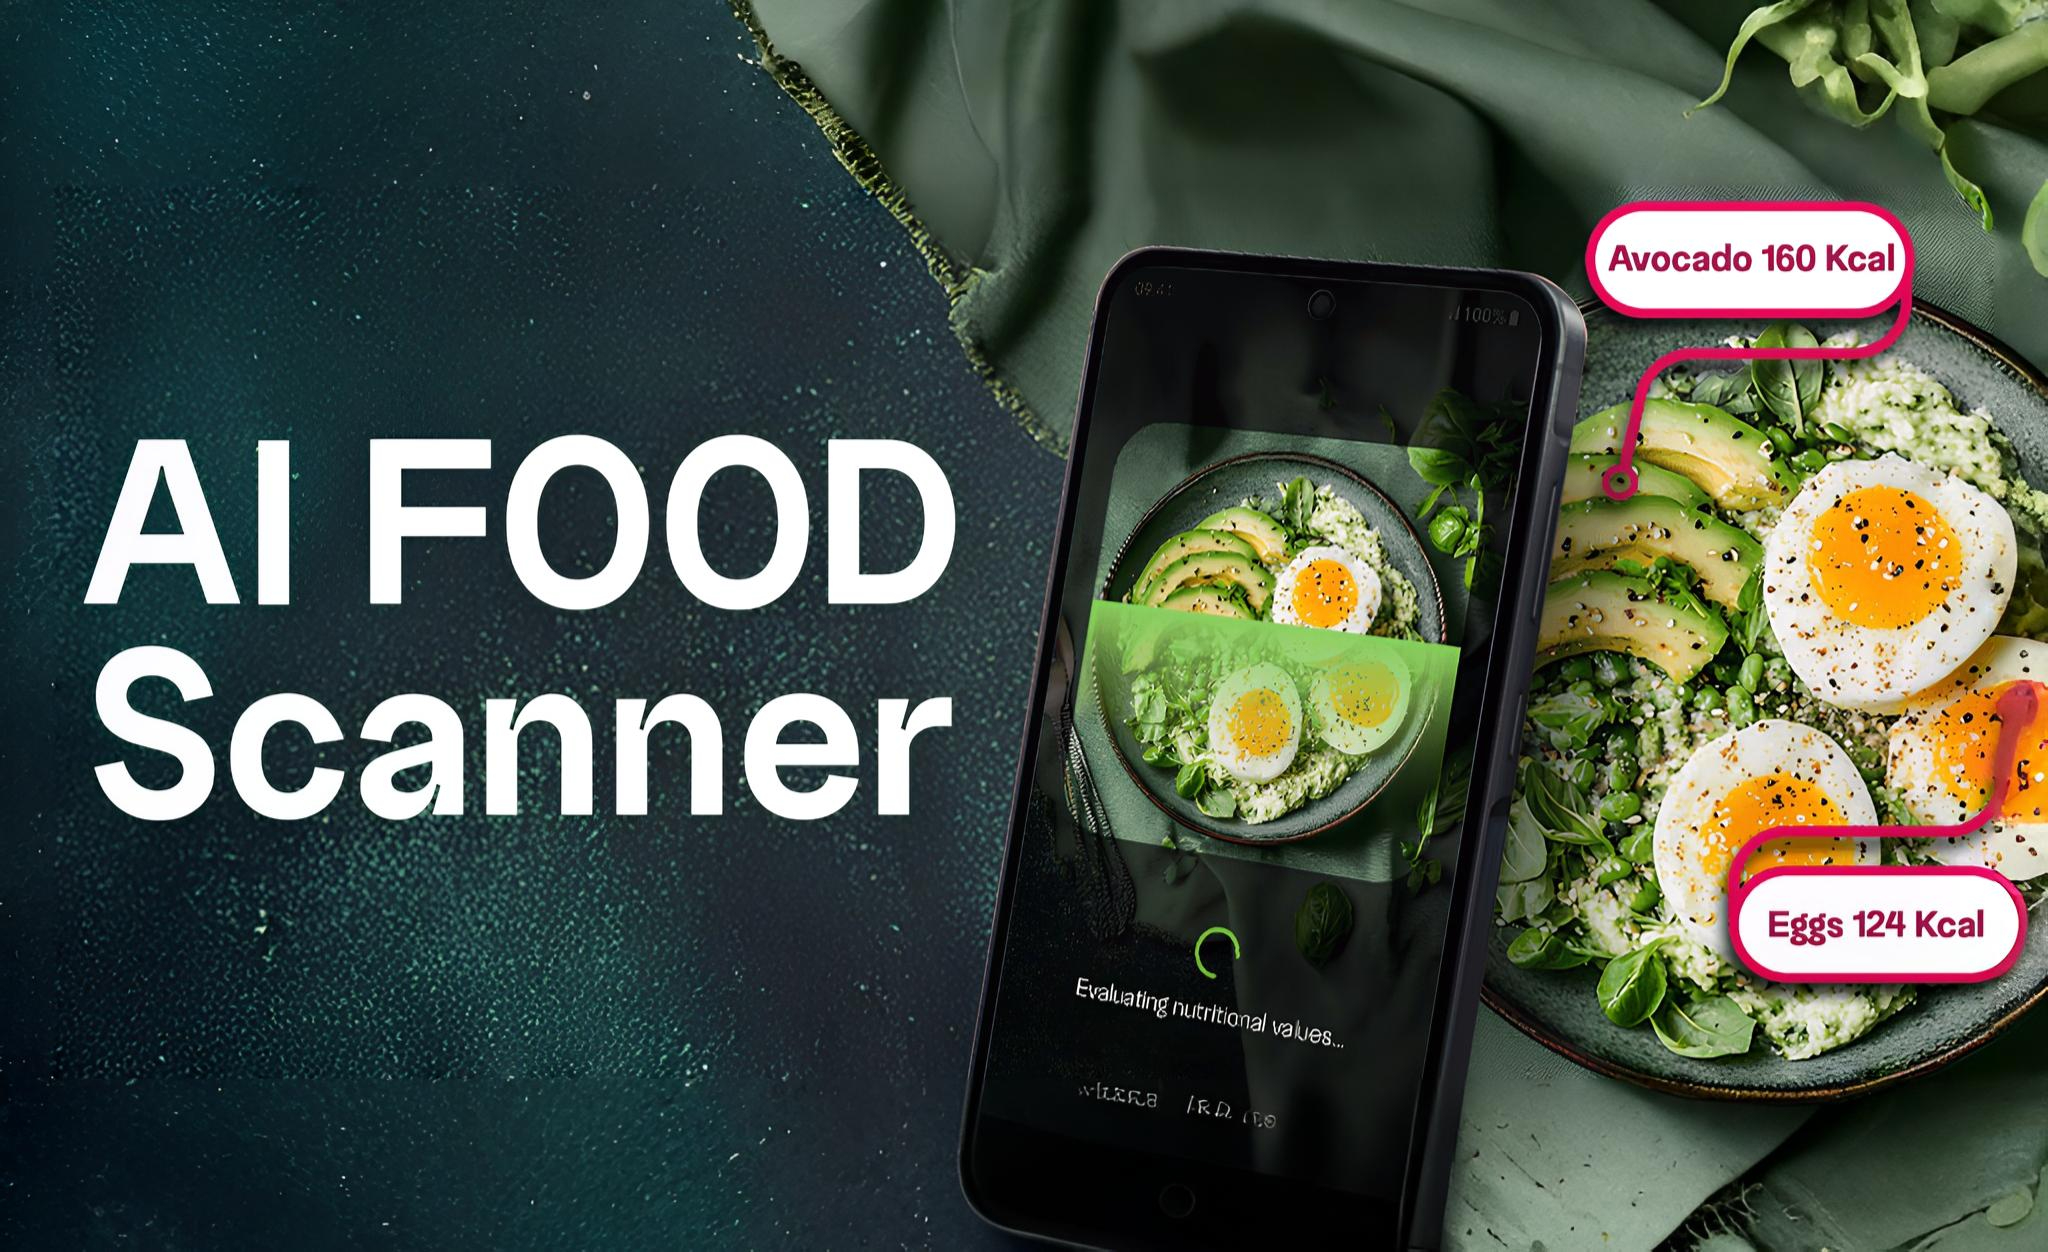
\includegraphics[width=0.9\textwidth]{../frontend/images/food_scanner.jpg}
\vspace{0.3cm}
\caption{PowerZone AI Food Scanner UI}
\end{figure}
\vspace{0.5cm}

\begin{figure}[h]
\centering
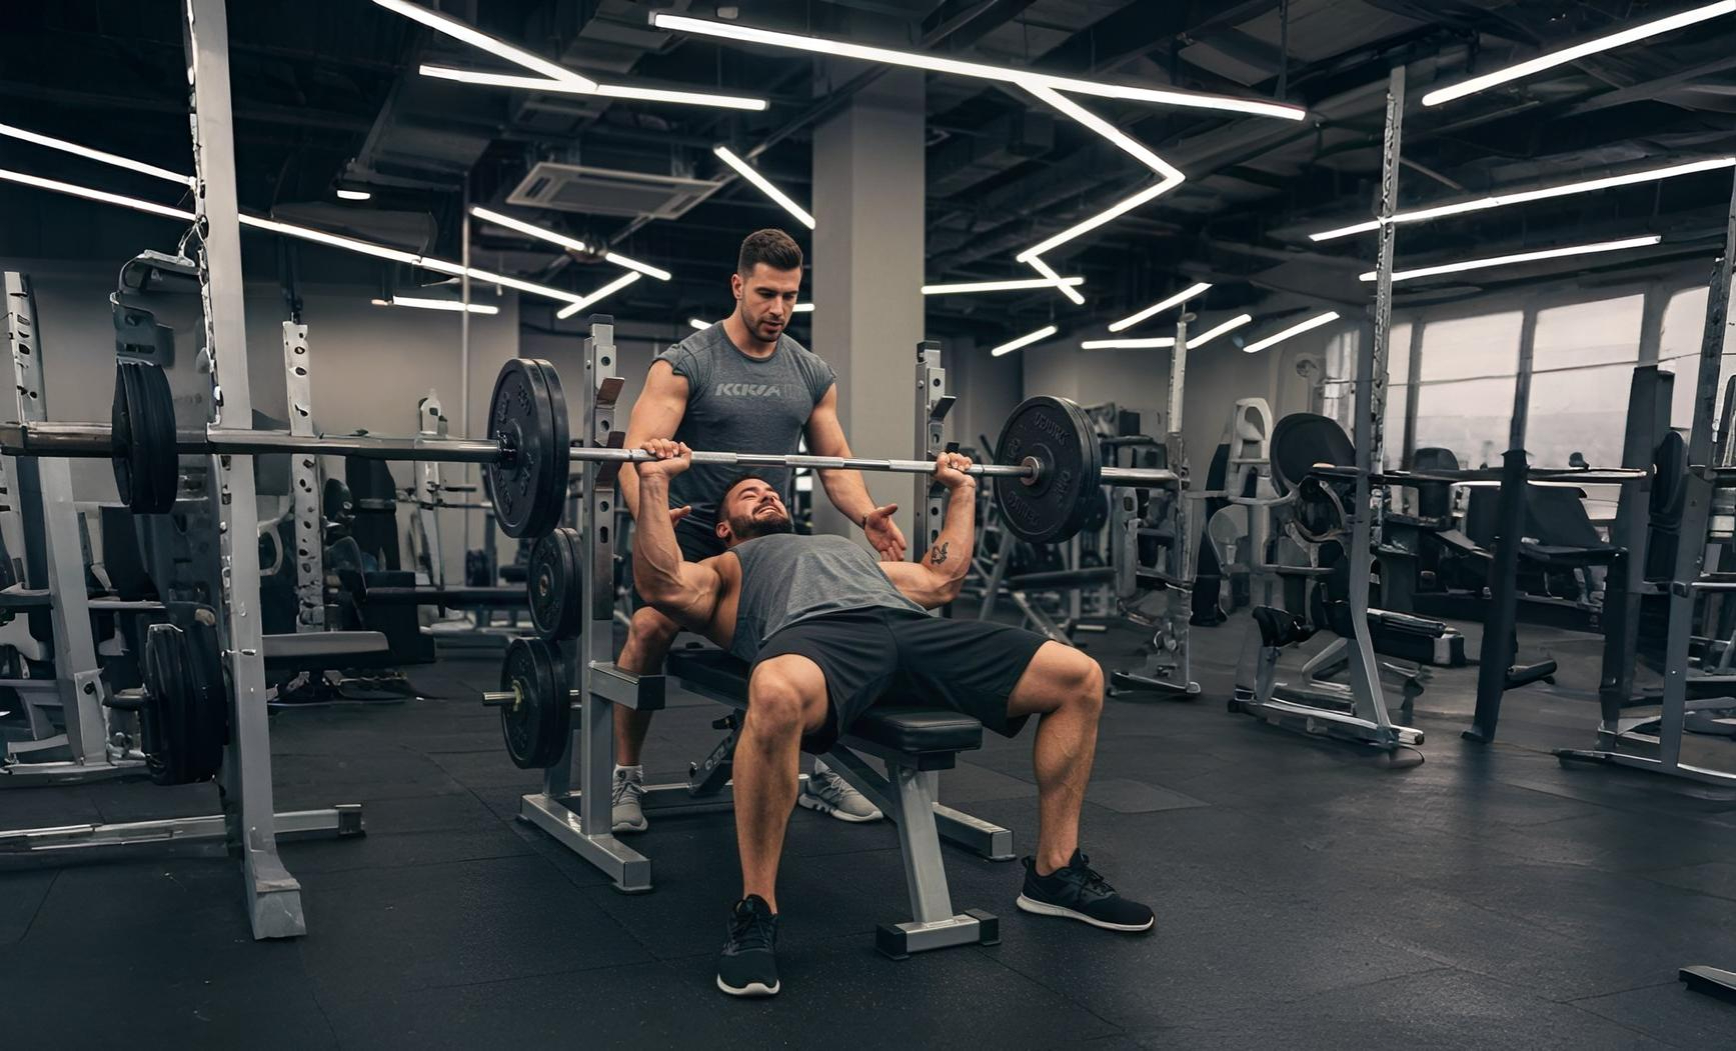
\includegraphics[width=0.9\textwidth]{../frontend/images/Fitness Coach.jpg}
\vspace{0.3cm}
\caption{PowerZone Fitness Coach Feature}
\end{figure}
\vspace{0.5cm}

\end{document}
